\externaldocument{report}
\section{Конструкторский раздел}

\subsection{Структура загрузочного модуля}
Точкой входа в драйвер и точкой выхода из драйвера являются функции из модуля \linuxpath{main.c}
\begin{lstlisting}
static int __init init_proc(void);
static void __exit exit_proc(void);
\end{lstlisting}
Соответствующие функции инициализации и деинициалдизации драйвера
вызываются из модуля \linuxpath{keyboard.c}:
\begin{lstlisting}
int init_keybrd(void);
void unreg_keybrd(void);
\end{lstlisting}
\newpar

Основной функцией драйвера-фильтра является функция \src{filter}:
\begin{lstlisting}
static bool filter(unsigned char data, unsigned char str, 
				   struct serio *serio);
\end{lstlisting}
Именно она выполняет все необходимые для фильтра функции:
\begin{itemize}
	\item Проверяет, нужно ли фильтровать входящий скан-код или нет;
	\item В случае, если фильтровать нужно, то обрабатывает входящий
		скан-код и возвращает \src{true} сообщая драйверу 
		\linuxcommand{i8042}, что скан-код уже обработан и дальнейшая
		обработка излишня;
	\item В случае, если скан-код обрабатывать не нужно никому, просто
		возвращает \src{true} и завершает работу. Эта ситуация
		может возникнуть, когда пришел скан-код отпущеной клавиши,
		которая потенциально должна быть обработана. В этом случае
		этот скан-код уже был обработан и дальнейшая обработка не 
		требуется.
	\item В случае, если скан-код не подлежит фильтрации, возвращается
		\src{false}.
\end{itemize}
В случае, если фильтр-функция возвращает \src{true}, драйвер \src{i8042} не станет
продолжать обработку пришедшего скан-кода. То есть его передача драйверу терминала осуществлена
не будет. В противном случае, если фильтр-функция вернет \src{false}, система сама продолжит обработку
пришедшего скан-кода.
\newpar

Основные структуры модуля локально описаны в файле \linuxpath{keyboard.c}:
\lstinputlisting[language=C, firstline=3, lastline=27, caption={}]{../src/keyboard.c}
Структура \src{key\_map} хранит в себе карту одной клавиши клавиатуры:
\begin{itemize}
	\item Поле \src{key} содержит код фильтруемой клавиши.
	\item Поле \src{codes} содержит массив кодов клавиш, которыми будет
		заменена фильтруемая клавиша. Для упрощения 
		кодирования кодов клавиш было принято, что если первый бит кода равен еденице, 
		то необходимо дополнительно послать код клавиши \key{Shift}. То есть, например,
		код \key{0x0b} является кодом клавиши \key{0}, в то время, как \key{0x8b} уже кодом
		клавиши \key{)}.
	\item Поле \src{count} содержит число значимых элементов в массиве \src{codes}.
\end{itemize}
Неименованная структура хранит в себе все необходимые для корректной работы модуля переменные:
\begin{itemize}
	\item Поле \src{current\_code\_index} содержит индекс последнего выведенного кода из массива
		\src{codes} структуры \src{key\_map}. В случае, если индекс становится больше значения 
		\src{count}, он обнуляется.
	\item Поле \src{last\_key} содержит значение последней нажатой клавиши, то есть значение поля
		\src{key} структуры \src{key\_map}.
	\item Поле \src{jiff} содержит значение переменной \src{jiffies}\footnote{Подробнее см. раздел~\ref{sec:jiffies}}
		на момент прерывания.
	\item Поле \src{key\_map} содержит массив из \src{KEYS\_COUNT} элементов, который определяет
		маску клавиш. Маска генерируется с помощью python-скрипта \linuxpath{key\_codes.py}\footnote{Подробнее см. \src{key\_codes.py --help}}
		и содержится в заголовочном файле \linuxpath{key\_map.h} в качестве макроса \src{KEY\_MAP}.
\end{itemize}

В файле \linuxpath{keyboard.h} заданы несколько определений, которые помогают более красиво организовать код:
\lstinputlisting[language=C, firstline=11, lastline=46, caption={}]{../src/keyboard.h}

\begin{itemize}
	\item Первые два определения (\src{I8042\_STR\_TIMEOUT} и {I8042\_STR\_PARITY}) были взяты из модуля
		\linuxpath{drivers/input/serio/i8042.h}  и используются для обработки статусного байта, который передается
		из модуля \linuxpath{i8042.c}.
	\item Макрос \src{KEY} позволяет макросу \src{KEY\_MAP} (который генерируется скриптом \linuxpath{key\_codes.py}) упростить 
		создание элемента структуры \src{struct key\_map}. Параметр \src{key}~-- ключевой код клавиши, параметр \src{\_count}~--
		число элементов в списке \src{\_codes}.
	\item \src{BTN\_PUSH} и \src{BTN\_POP} позволяют создать мнемоническую интерпретацию для определения того, код какой
		клавиши был прислан: нажатой или отжатой.
	\item \src{IS\_SHIFT}, \src{SHIFT} и \src{RM\_SHIFT} используются для определения и управления регистром символа. Конкретнее,
		эти макроподстановки используются при анализе \src{key\_map.codes}.
	\item \src{BACKSPACE\_KEY} и \src{SHIFT\_KEY} создают мнемонические константы для кодов клавиш \key{Backspace} и 
		\key{Shift} соответственно.
	\item \src{IS\_KEYBRD}, \src{IS\_EXTRA\_KEY} и \src{IS\_IGNORE} представляют собой
		набор условных макрооператоров, которые позволяют на основе входного параметра определить:
		\begin{itemize}
			\item соответствует ли статусная строка, переданная в первое макроопределение, клавиатуре, или нет
			\item является ли байт, переданный во второе макроопределение статусным или нет. Возвращает
				\src{true}, например, если была нажата\\клавиша \key{Стрелка~вверх}
			\item нужно ли переданный байт проигнорировать, или нет. Этот байт может прийти от контроллера
				в случае, если произошла какая то ошибка, например был считан скан-код неизвестной системной клавиши
		\end{itemize}
	\item \src{STR\_TO\_DFL}~-- макрос для преобразования статусной строки из вида понятного для модуля \src{i8042} в
		вид понятный модулю \src{serio}. Макрос был скопирован из модуля \src{i8042}.
	\item \src{send\_key}~-- макрос для посылки подсистеме ввода нужного для драйвера-фильтра кода клавиши.\\
		\src{serio}~-- адрес структуры типа \src{struct serio}, который передается в фильтр модулем \src{i8042};\\
		\src{data}~-- байт (переменная типа \src{unsigned char}), который передается подсистеме ввода;\\
		\src{flags}~-- статусная строка, которая передается в необработанном виде из модуля \src{i8042} и которая
			требует обработки с помощью макроса \src{STR\_TO\_DFL}.
\end{itemize}

\subsection{Структура \src{Makefile}'а}
\linuxutil{make}~--- утилита, автоматизирующая процесс преобразования файлов из одной формы в другую. Чаще всего 
это компиляция исходного кода в объектные файлы и последующая компоновка в исполняемые файлы или библиотеки.
\newpar

В рассматриваемом проекте \src{Makefile} применяется для компиляции исходного кода драйвера в загружаемый модуль ядра, а 
так же для генерации карты необходимых клавиш клавиатуры.
\newpar

Первая его половина составляет набор определений для более гибкой и удобной сборки.
Вторая его часть составляет набор целей для построения и очистки проекта.
\newpar

При запуске \src{default}-цели, перед тем как начать сборку модуля,
программа \src{make} должна запустить генерацию файла \src{key\_map.h}.
Этот файл генерируется скриптом \src{key\_codes.py}, который использует
\src{key\_map.conf} в качестве конфигурационного файла.
\newpar

Для того, чтобы сформировать \src{Debug}-сборку проекта необходимо в 
переменную \src{DEFINES} \src{Makefile}'а включить строку <<\src{DEBUG,}>> (наличие запятой обязательно) 
и пересобрать весь проект. Это действие создаст макроопределение \src{DEDUG} в проекте, что приведет
к созданию набора вспомогательных макроопределний, которые помогут выносить в 
лог-файл необходимую для отладки информацию. В частности, по умолчанию, при
определенном \src{DEBUG} включается логирование каждой нажатой клавиши, которая 
должна быть в дальнейшем обработана.
При этом, в лог-файл выводится информация как о нажатии клавиши, так и о ее отжатии, а 
так же и значение статусного регистра. Все значения отображены в шестнадцатиричном виде.
Пример вывода отладочной информации в лог-файл (может быть получена с помощью комманды
\linuxcommand{dmesg~|~grep dFilter} в командной оболочке ОС \linux):
\begin{verbatim}
[11661.204828] dFilter notice: Loading driver...
[11661.204836] dFilter notice: Driver loaded
[11661.297068] dFilter notice: data: 0x9c; str: 0x15
[11663.959559] dFilter notice: data: 0x48; str: 0x15
[11664.424872] dFilter notice: data: 0x48; str: 0x15
[11665.059146] dFilter notice: data: 0x47; str: 0x15
........
[11735.202478] dFilter notice: data: 0xf; str: 0x15
[11735.223780] dFilter notice: data: 0xa6; str: 0x15
[11735.298248] dFilter notice: data: 0x8f; str: 0x15
[11735.571320] dFilter notice: data: 0x1c; str: 0x15
[11735.587842] dFilter notice: Stopping driver...
[11735.587852] dFilter notice: Driver stopped
\end{verbatim}

\subsection{Генерация маски клавиш}
Генерация маски клавиш осуществляется скриптом \linuxpath{key\_codes.py}.
Скрипт написан на языке высокого уровня Python v.\,3.3.2.
Основной функцией скрипта является отображение маски клавиш на экран в 
удобном для пользователя формате.
\newpar

\verbfilebox{sample_user_output}

\begin{figure}[h!]
\centering
\theverbbox
\caption*{Пример отображения маски клавиш}
\end{figure}

\par Для более удобного пользования и для более полной имитации клавиатуры кнопочного телефона,
была произведена вертикальная инверсия цифровых символов.
\newpar

Второй функцией скрипта \linuxpath{key\_codes.py} является генерация заголовочного
файла \linuxpath{key\_map.h}, который подключается к файлу \linuxpath{keyboard.h} и содержит
макроконструкцию для формирования массива \src{struct key\_map key\_map[]}.
Скрипт так же просчитывает максимальное число элементов в маске и число масок и записывает
их в макроопределения \src{MAX\_CODES} и \src{KEYS\_COUNT} соответственно.
\newpar

Таким образом, один скрипт позволяет с помощью одного и того же файла конфигурации
сформировать идентичные маски символов, которые будут использоваться как в самом драйвере,
так и для информирования пользователя о текущей конфигурации дополнительной цифровой клавиатуры.
\vspace*{\fill}
\newpage
\subsection{Алгоритм работы}
\begin{figure}[h]
	\centering
	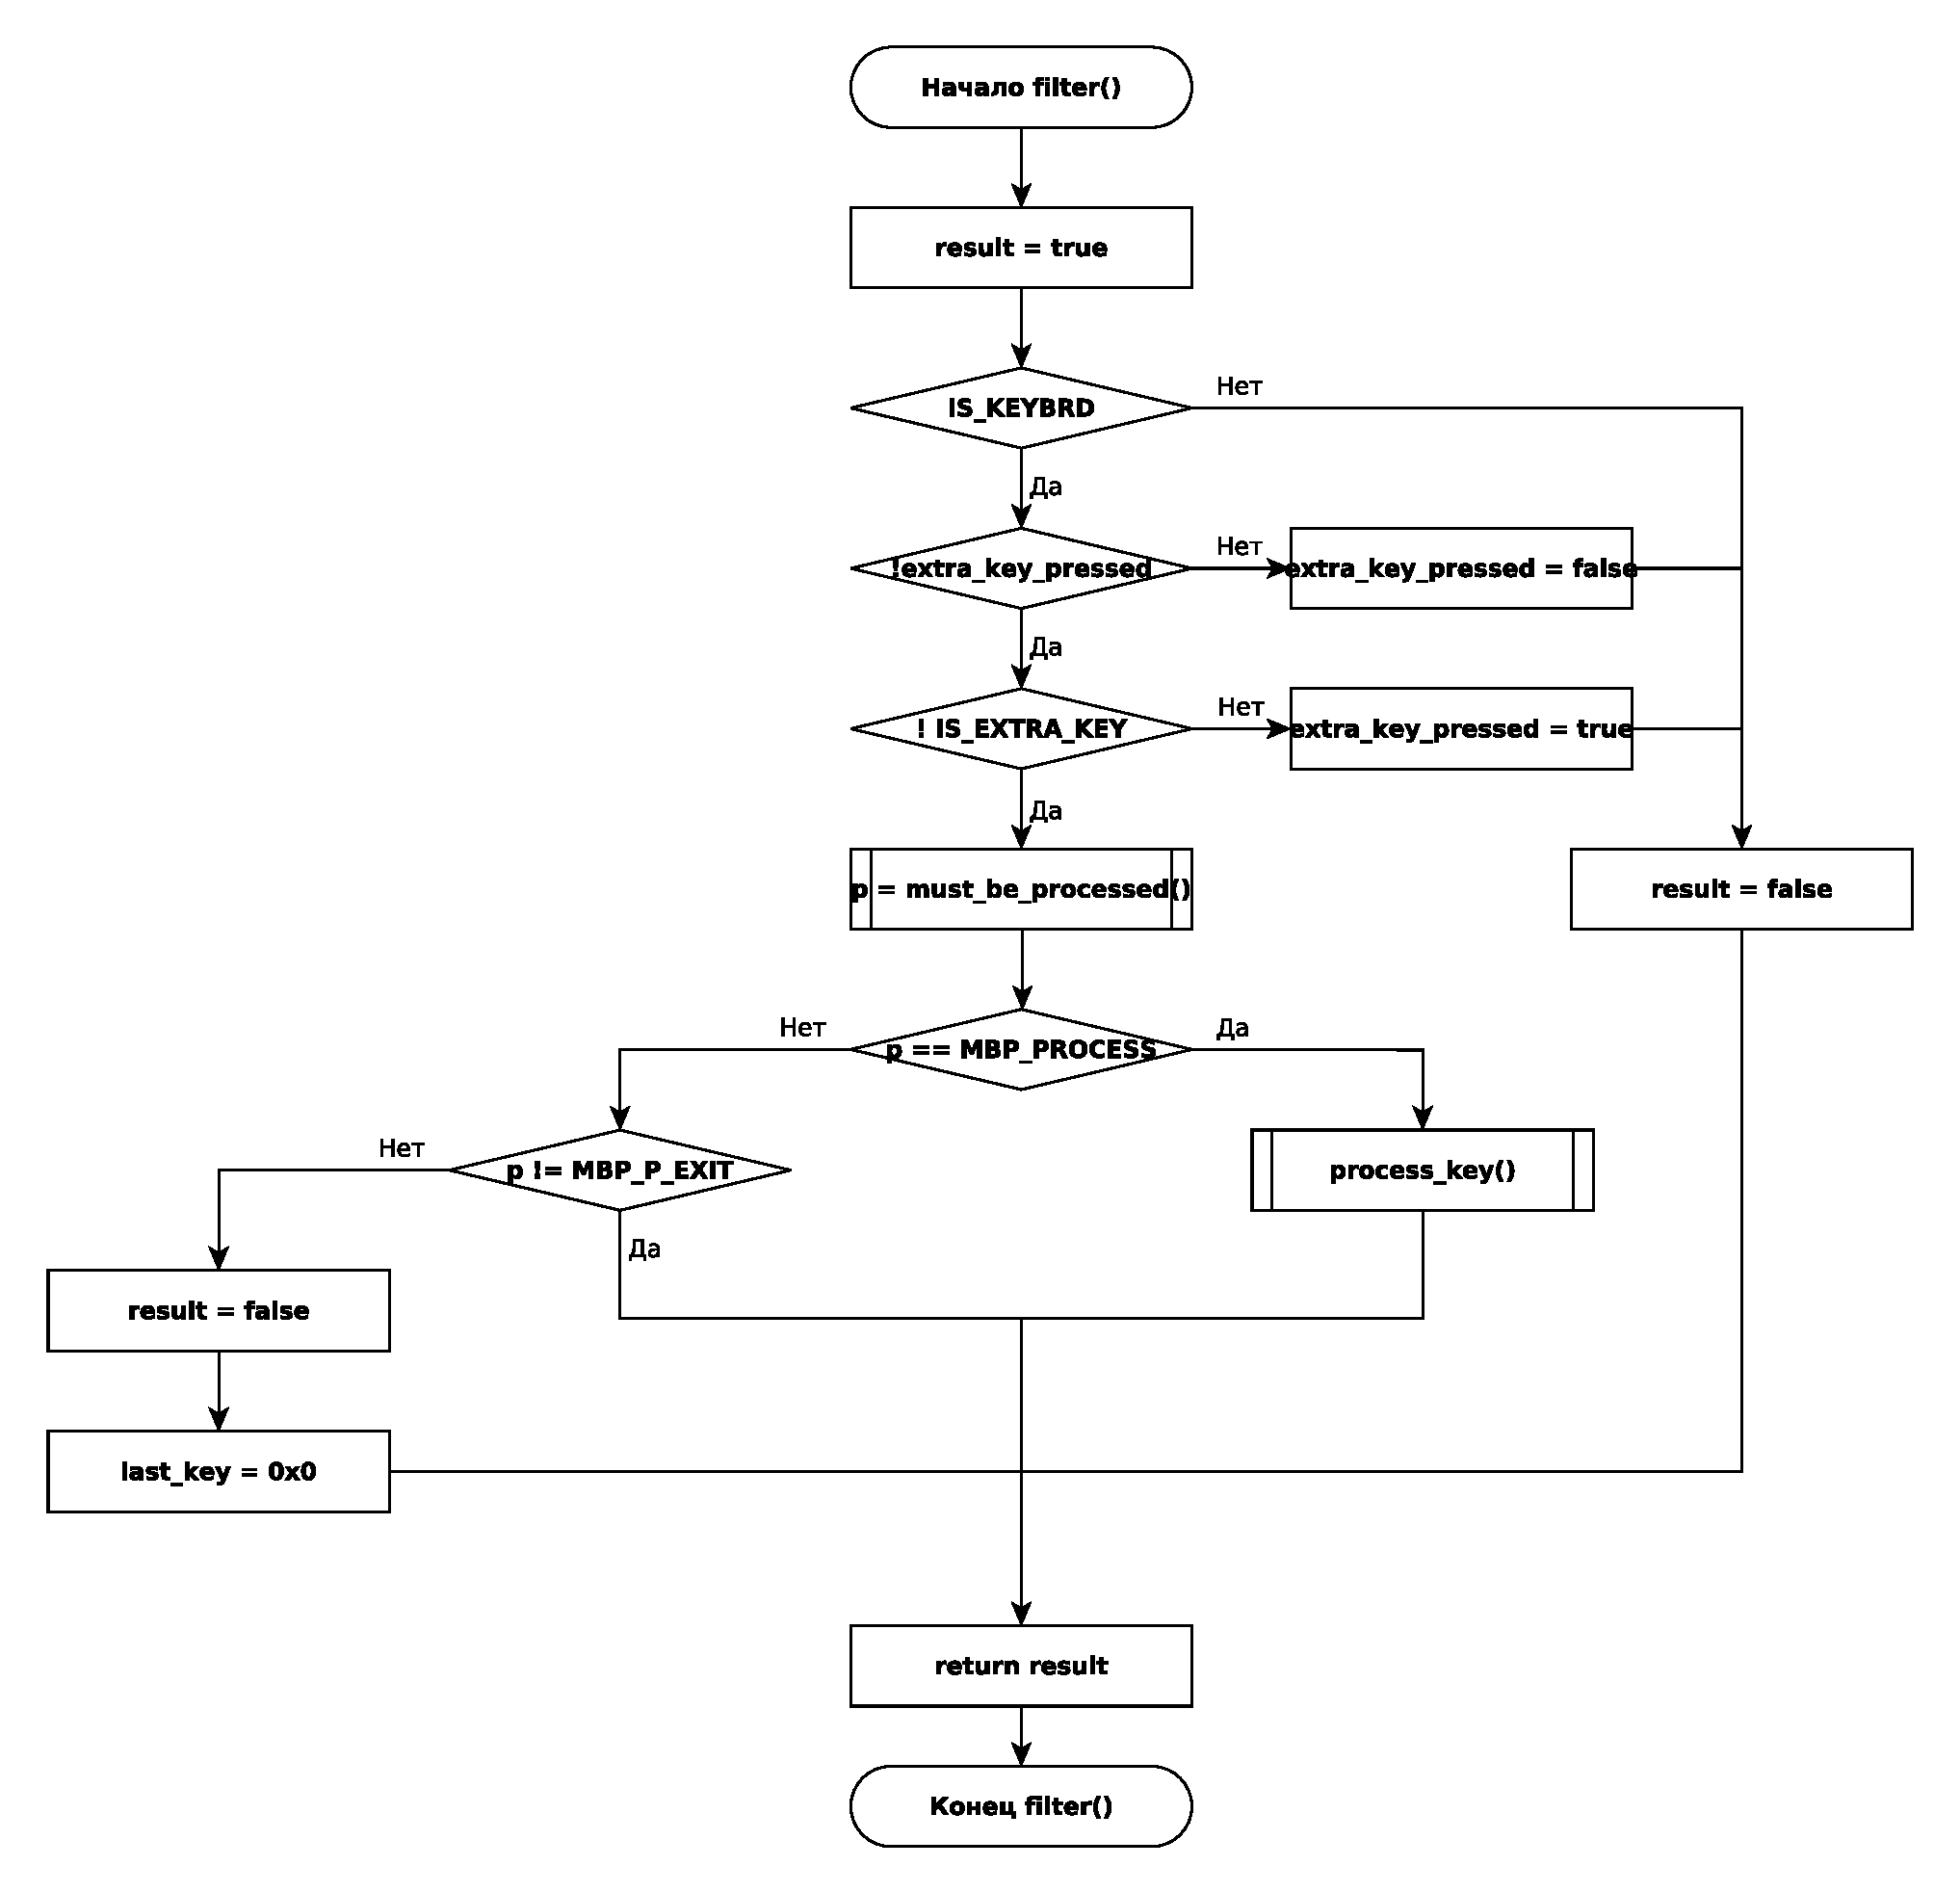
\includegraphics[scale=0.5]{filter.eps}
	\caption*{Алгоритм работы функции filter()}
\end{figure}
\begin{figure}[p]
	\centering
	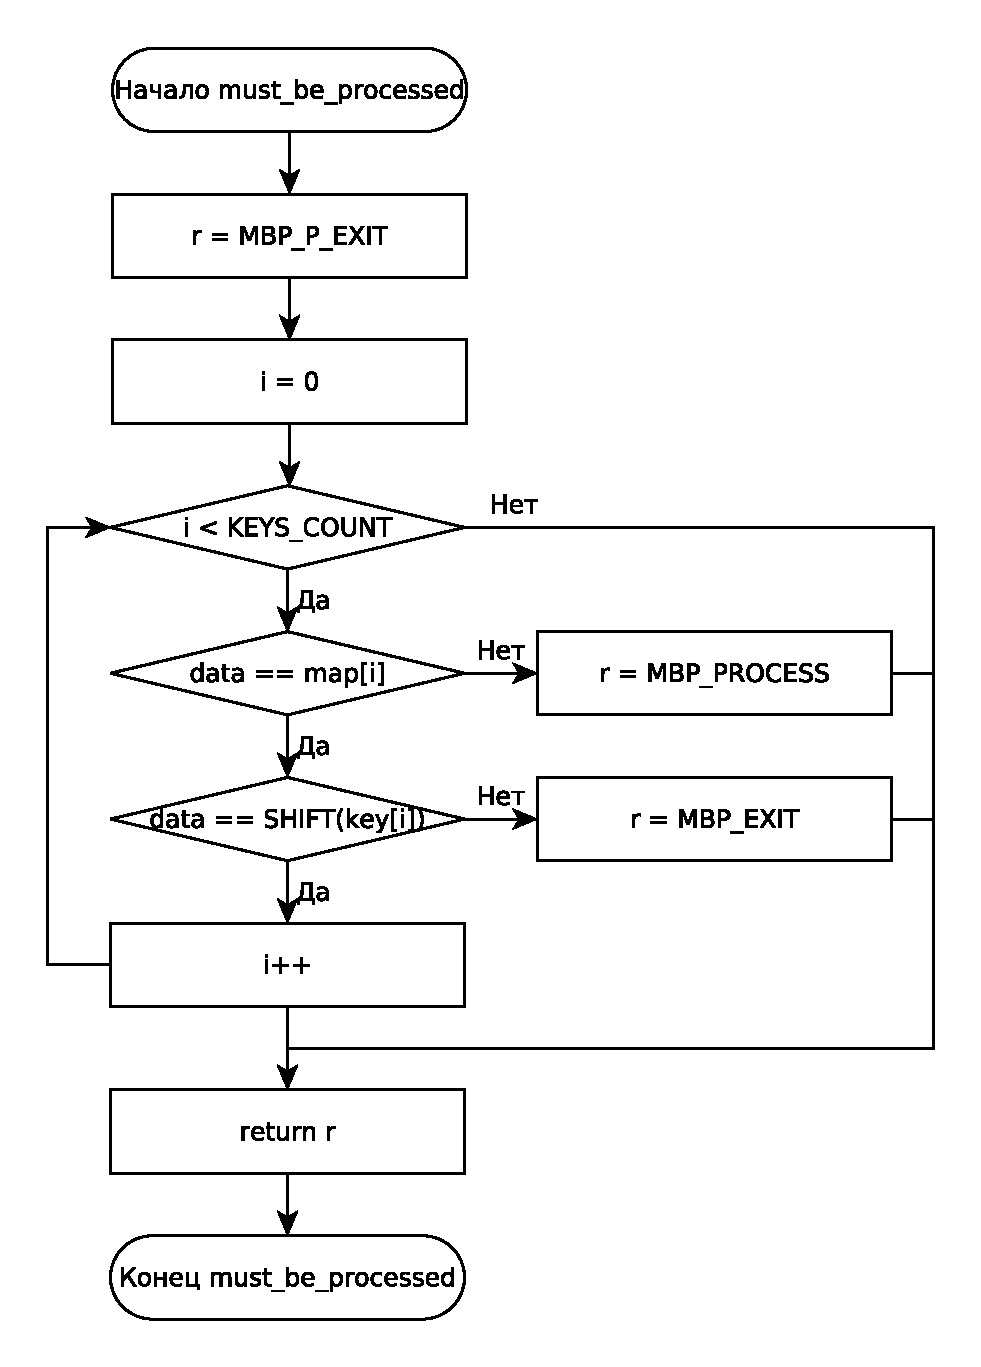
\includegraphics[scale=0.5]{must_be_processed.eps}
	\caption*{Алгоритм работы функции must\_be\_processed()}
\end{figure}
\newgeometry{top=1.5cm}
\begin{figure}[p]
	\centering
	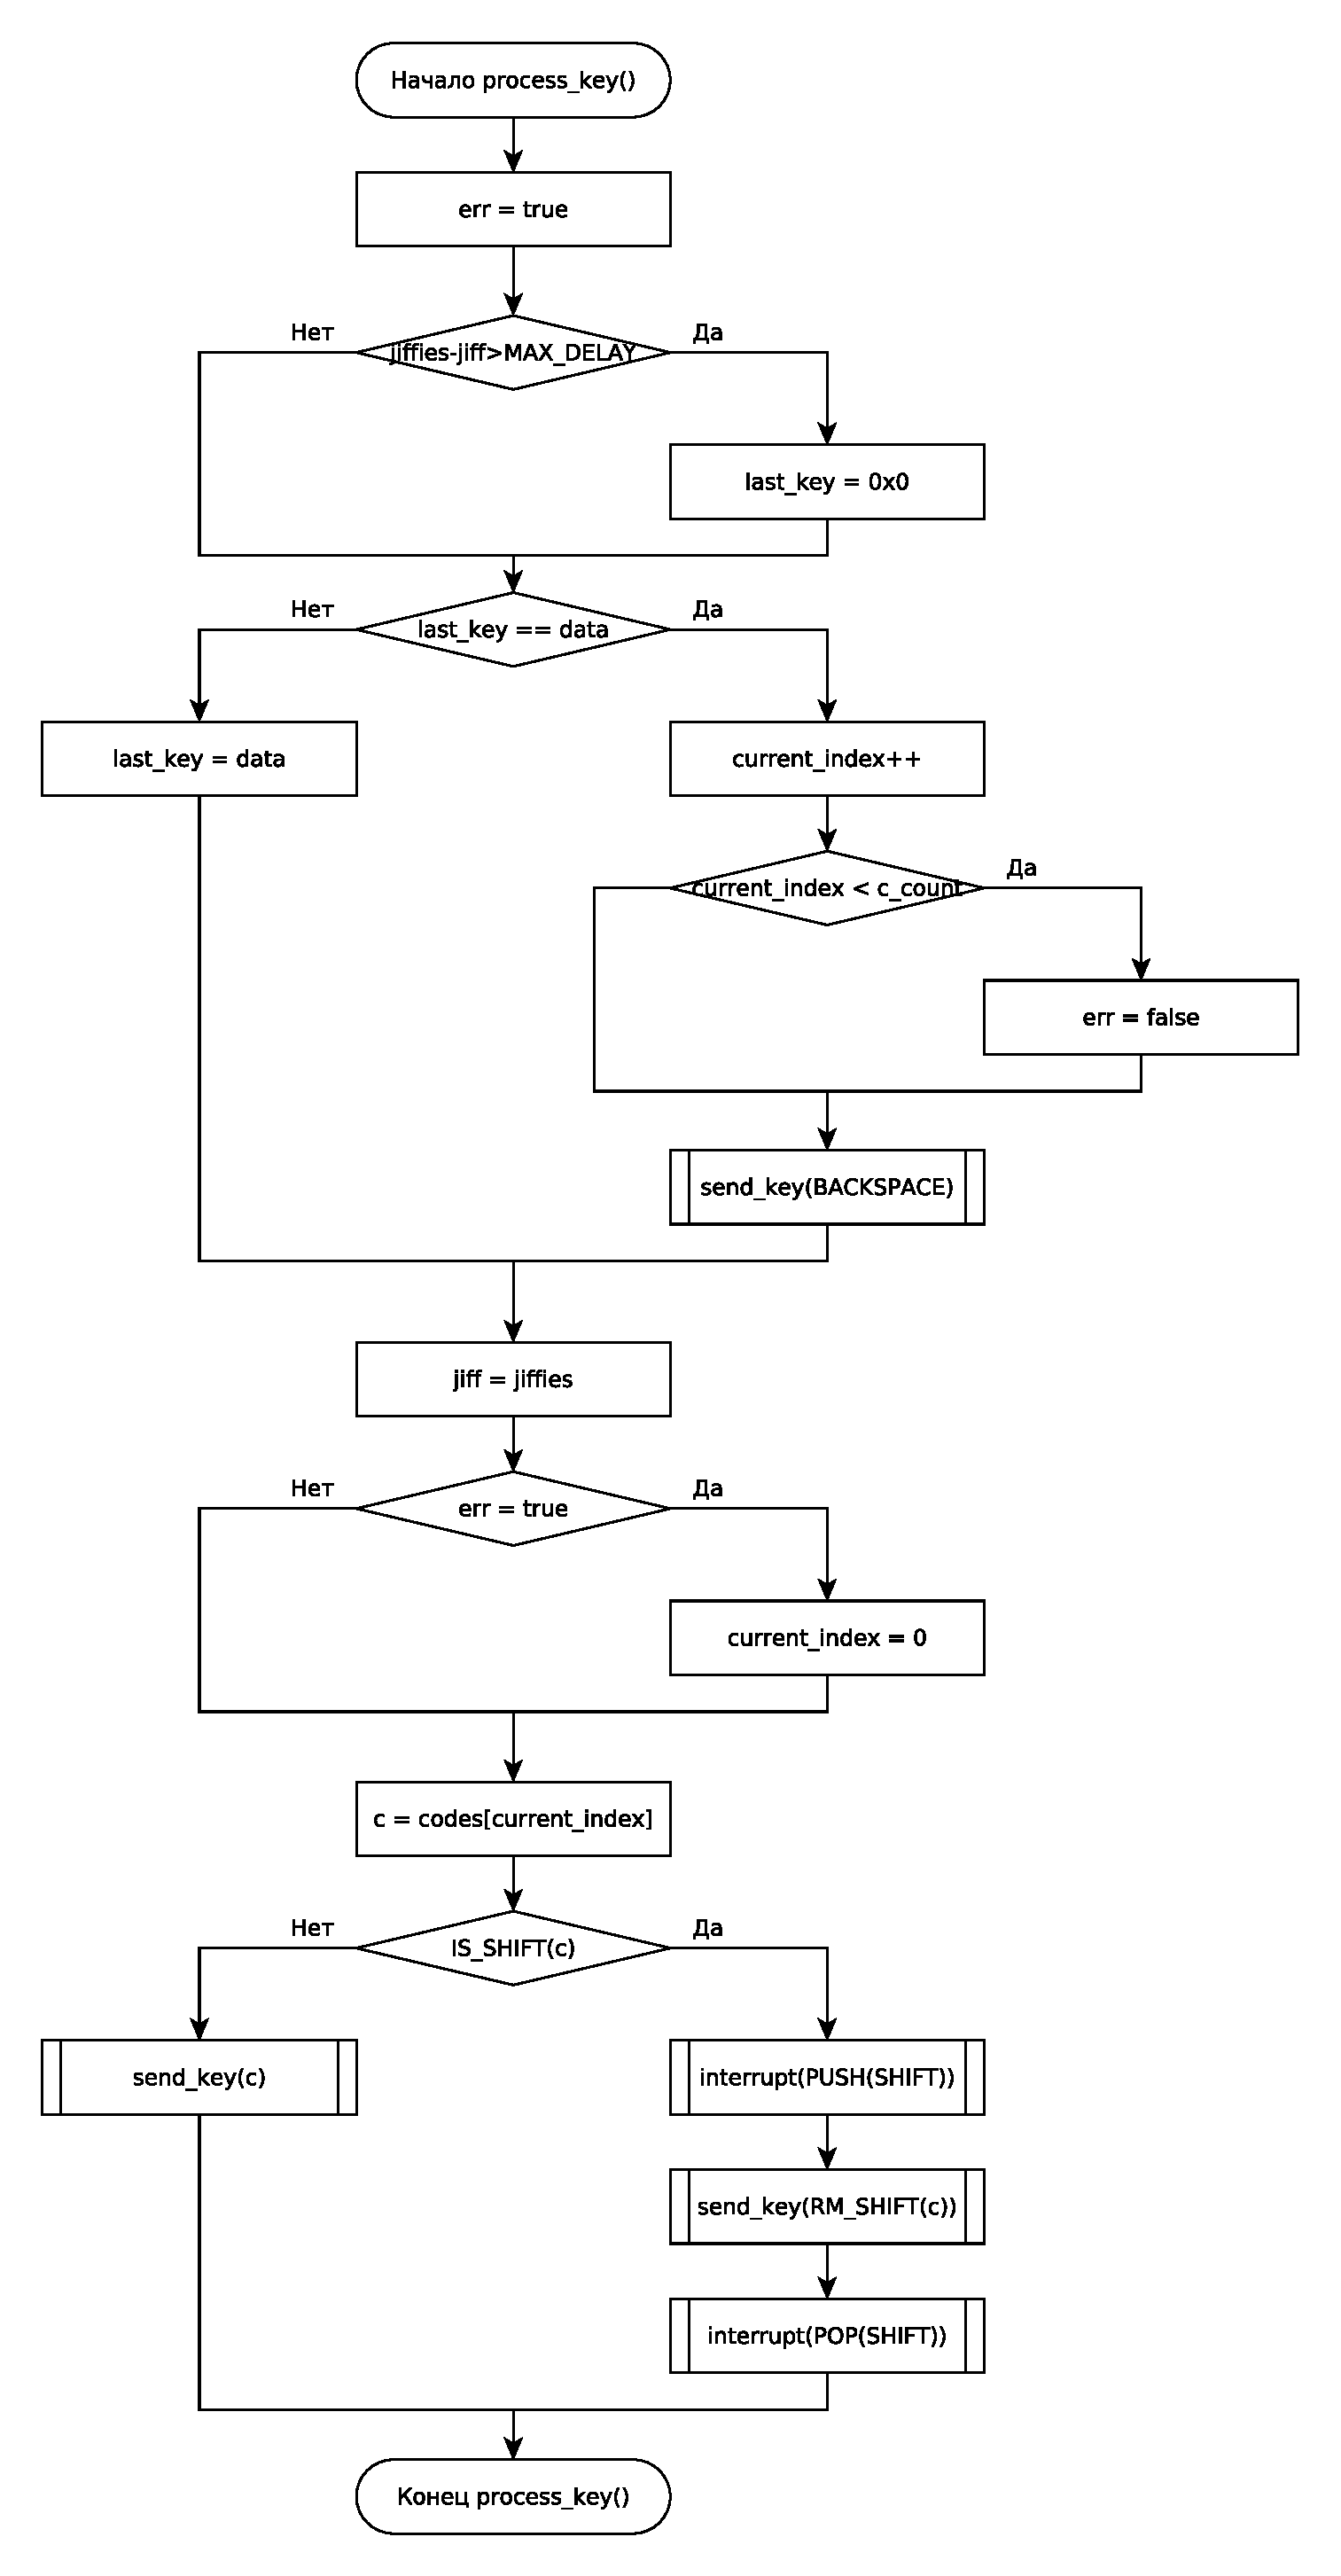
\includegraphics[scale=0.5]{process_key.eps}
	\caption*{Алгоритм работы функции process\_key()}
\end{figure}
\restoregeometry
\newpage
